\documentclass[aspectratio=169,10pt]{beamer}

% ─── Theme ───────────────────────────────────────────────────────────────────
\usetheme{Madrid}
\usecolortheme{seahorse}
\setbeamertemplate{navigation symbols}{}
\setbeamertemplate{footline}[frame number]
\setbeamerfont{frametitle}{size=\large,series=\bfseries}
\setbeamerfont{title}{size=\Large,series=\bfseries}

% ─── Packages ────────────────────────────────────────────────────────────────
\usepackage{amsmath,amssymb,mathtools}
\usepackage{graphicx}
\usepackage{booktabs}
\usepackage{xcolor}
\usepackage{tikz}
\usepackage{pgfplots}
\pgfplotsset{compat=1.17}
\usepackage{multicol}
\usepackage{tcolorbox}
\tcbuselibrary{skins,breakable}
\usepackage{fontawesome5}

% ─── Colors ──────────────────────────────────────────────────────────────────
\definecolor{stanford}{RGB}{140,21,21}
\definecolor{physgreen}{RGB}{39,174,96}
\definecolor{basered}{RGB}{231,76,60}
\definecolor{stepA}{RGB}{142,68,173}
\definecolor{stepB}{RGB}{41,128,185}
\definecolor{stepC}{RGB}{39,174,96}
\definecolor{stepD}{RGB}{230,126,34}
\definecolor{darkgray}{RGB}{44,62,80}

\setbeamercolor{frametitle}{bg=stanford,fg=white}
\setbeamercolor{title}{fg=stanford}
\setbeamercolor{structure}{fg=stanford}
\setbeamercolor{block title}{bg=stanford,fg=white}

% ─── Custom boxes ─────────────────────────────────────────────────────────────
\newtcolorbox{physbox}[2][]{
  enhanced,colback=#1!10,colframe=#1,
  title={\textbf{#2}},fonttitle=\small\bfseries,
  left=3pt,right=3pt,top=2pt,bottom=2pt,
  boxrule=1.2pt
}

% ─── Commands ────────────────────────────────────────────────────────────────
\newcommand{\physcot}{\textsc{PhysCoT}}
\newcommand{\openvla}{\textsc{OpenVLA}}
\newcommand{\ecot}{\textsc{ECoT}}
\newcommand{\succ}[1]{\textcolor{physgreen}{\textbf{#1}}}
\newcommand{\fail}[1]{\textcolor{basered}{\textbf{#1}}}

% ─── Title ────────────────────────────────────────────────────────────────────
\title[\physcot{}]{%
  \physcot{}: Physics-Intuitive Chain-of-Thought\\
  Prompting for Robot Manipulation with \openvla{}
}
\author{Bobby Shi}
\institute{Stanford University \\ \texttt{shi02@stanford.edu}}
\date{CS 372 Final Project · March 2026}

% ─────────────────────────────────────────────────────────────────────────────
\begin{document}
% ─────────────────────────────────────────────────────────────────────────────

% ── Slide 1: Title ──────────────────────────────────────────────────────────
\begin{frame}
\titlepage
\vspace{-0.3cm}
\begin{center}
\small
\textbf{Code:} \url{https://github.com/bobbyshi/physcot} [placeholder]
\end{center}
\end{frame}

% ── Slide 2: Motivation ──────────────────────────────────────────────────────
\begin{frame}{Motivation: Why Physics Reasoning for Manipulation?}
\begin{columns}[T]
\column{0.55\textwidth}
\textbf{The problem with reactive VLA policies:}
\begin{itemize}
  \item \openvla{}, RT-2 map observation $\to$ action directly
  \item No explicit reasoning about \emph{physical consequences}
  \item Fail on tasks where physics intuition is required:
    \begin{itemize}
      \item Where to push a block to topple vs.\ slide?
      \item Which tool can reach around an obstacle?
    \end{itemize}
\end{itemize}

\vspace{0.4cm}
\textbf{Generic CoT is not enough:}
\begin{tcolorbox}[colback=basered!10,colframe=basered,left=3pt,right=3pt,
                  top=2pt,bottom=2pt,boxrule=1pt]
\small
``Think step by step'' $\to$ vague, non-physical,\\
not grounded in contact mechanics.
\end{tcolorbox}

\column{0.42\textwidth}
\begin{center}
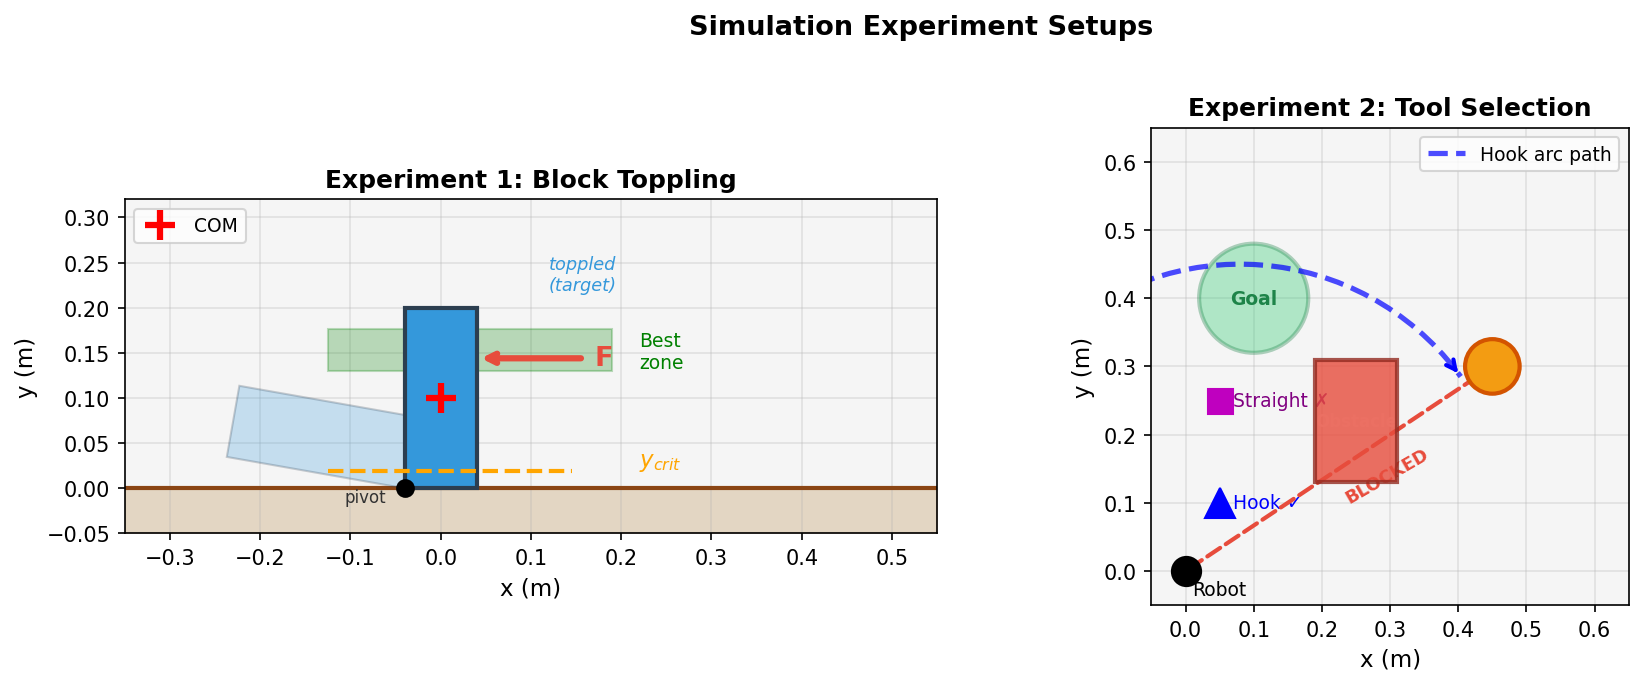
\includegraphics[width=\linewidth]{../results/figures/fig_exp_setup.png}
\end{center}
\small Two tasks that \emph{require} physical reasoning to succeed.
\end{columns}
\end{frame}

% ── Slide 3: ECoT inspiration and gap ───────────────────────────────────────
\begin{frame}{Inspiration: ECoT — and What We Add}
\begin{columns}[T]
\column{0.48\textwidth}
\textbf{\ecot{} (Zawalski et al., 2024):}
\begin{itemize}
  \item Trains VLA to produce reasoning tokens before actions
  \item Reasoning: sub-goals, scene description, motion plan
  \item Improves performance and interpretability
  \item \textbf{Requires supervised finetuning}
\end{itemize}

\vspace{0.3cm}
\textbf{Gap we target:}
\begin{itemize}
  \item \ecot{} reasoning is generic (not physics-specific)
  \item Training data is expensive
  \item \textbf{Can physics-intuitive reasoning work at inference time only?}
\end{itemize}

\column{0.48\textwidth}
\textbf{\physcot{} (ours):}
\begin{itemize}
  \item \succ{No training} — pure prompting
  \item Reasoning is \textbf{explicitly physics-aware}:
    \begin{itemize}
      \item Torque, friction, stability
      \item Tool affordance, geometry
      \item Visual physical estimates
    \end{itemize}
  \item Same schema across all tasks
\end{itemize}

\vspace{0.3cm}
\begin{tcolorbox}[colback=physgreen!10,colframe=physgreen,left=3pt,right=3pt,
                  top=2pt,bottom=2pt,boxrule=1pt]
\small
\textbf{Key claim:} physics-intuitive, visually grounded,
action-consequential reasoning is what manipulation needs.
\end{tcolorbox}
\end{columns}
\end{frame}

% ── Slide 4: PhysCoT key idea ────────────────────────────────────────────────
\begin{frame}{\physcot{}: The Key Idea}
\begin{center}
\large
At every decision step, reason in \textbf{four physics-specific stages}:
\end{center}

\vspace{0.3cm}
\begin{columns}[T]
\column{0.24\textwidth}
\begin{tcolorbox}[colback=stepA!12,colframe=stepA,title={\small Step A},
                  left=3pt,right=3pt,top=2pt,bottom=2pt,boxrule=1.2pt]
\small\textbf{Task Decomp.}\\[3pt]
Overall goal\\
Immediate sub-goal\\
Required state change
\end{tcolorbox}

\column{0.24\textwidth}
\begin{tcolorbox}[colback=stepB!12,colframe=stepB,title={\small Step B},
                  left=3pt,right=3pt,top=2pt,bottom=2pt,boxrule=1.2pt]
\small\textbf{Relevant Physics}\\[3pt]
Torque / leverage\\
Friction regime\\
Stability / affordance
\end{tcolorbox}

\column{0.24\textwidth}
\begin{tcolorbox}[colback=stepC!12,colframe=stepC,title={\small Step C},
                  left=3pt,right=3pt,top=2pt,bottom=2pt,boxrule=1.2pt]
\small\textbf{Visual Estimates}\\[3pt]
COM location\\
Aspect ratio\\
Tool geometry / path
\end{tcolorbox}

\column{0.24\textwidth}
\begin{tcolorbox}[colback=stepD!12,colframe=stepD,title={\small Step D},
                  left=3pt,right=3pt,top=2pt,bottom=2pt,boxrule=1.2pt]
\small\textbf{Action Impl.}\\[3pt]
Contact point\\
Direction \& force\\
Causal rationale
\end{tcolorbox}
\end{columns}

\vspace{0.4cm}
\begin{center}
\begin{tikzpicture}[font=\small]
  \foreach \i/\c/\l in {
    0/stepA/A, 1/stepB/B, 2/stepC/C, 3/stepD/D}{
    \node[draw=\c,fill=\c!20,rounded corners=3pt,
          minimum width=1.4cm,minimum height=0.6cm,
          very thick] at (\i*2.2,0) {\textbf{Step \l}};
  }
  \foreach \i in {0,1,2}{
    \draw[->,very thick,darkgray] (\i*2.2+0.7,0) -- (\i*2.2+1.5,0);
  }
  \draw[->,very thick,darkgray] (6.7+0.7,0) -- (8.5,0);
  \node[draw=darkgray,fill=darkgray!15,rounded corners=3pt,
        minimum width=1.5cm,minimum height=0.6cm,
        very thick] at (9.2,0) {\textbf{Action}};
\end{tikzpicture}
\end{center}
\end{frame}

% ── Slide 5: Method pipeline ─────────────────────────────────────────────────
\begin{frame}{Method Pipeline}
\begin{center}
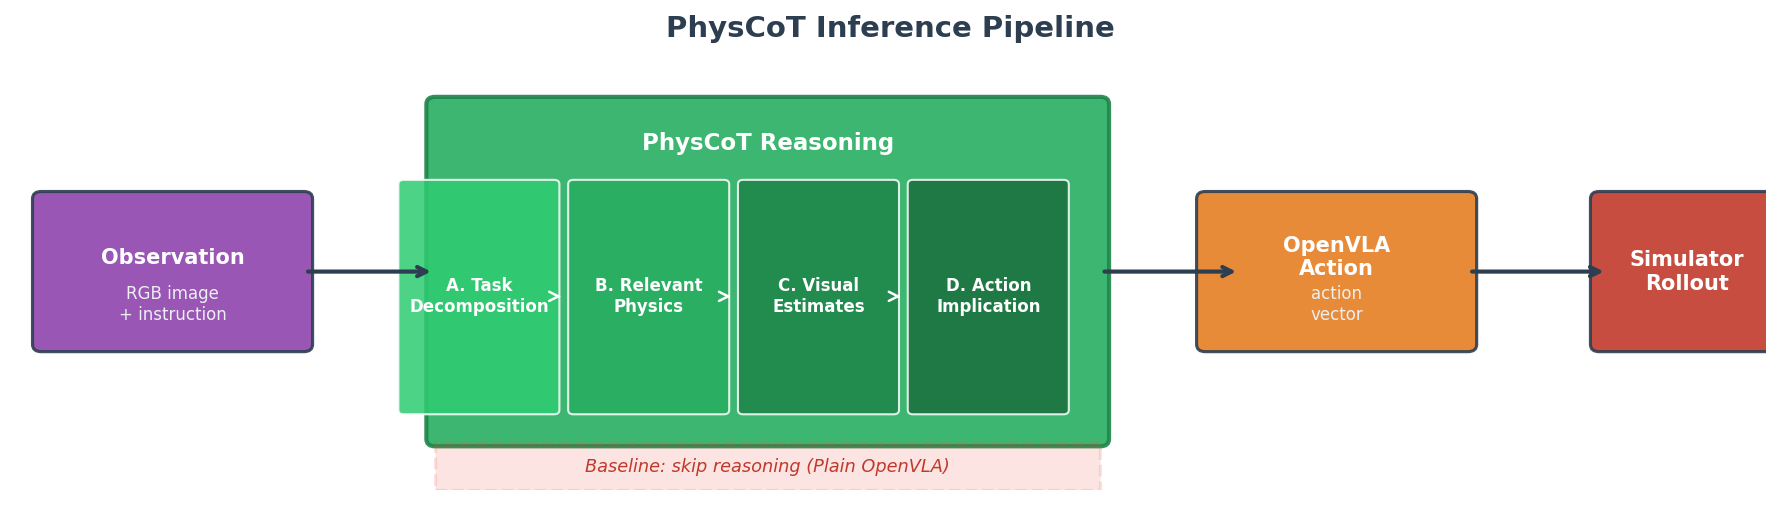
\includegraphics[width=0.95\linewidth]{../results/figures/fig_pipeline.png}
\end{center}
\vspace{0.2cm}
\small
\begin{itemize}
  \item \textbf{Baseline}: observation $\to$ \openvla{} action (no reasoning)
  \item \textbf{\physcot{}}: observation $\to$ 4-step physics reasoning $\to$ \openvla{} action
  \item \textbf{No weights changed} — pure inference-time prompting
\end{itemize}
\end{frame}

% ── Slide 6: Experiment 1 setup ──────────────────────────────────────────────
\begin{frame}{Experiment 1: Block Toppling}
\begin{columns}[T]
\column{0.52\textwidth}
\textbf{Task:} Push upright block so it topples ($\theta > 60°$)

\vspace{0.3cm}
\textbf{Key physics:}
\[
  \tau_\text{push} = F \cdot y_c \quad>\quad \tau_\text{crit} = mg\frac{w}{2}
\]
\[
  \Rightarrow \quad y_c > y_c^* = \frac{mgw}{2F}
\]

\vspace{0.2cm}
\textbf{Baseline}: pushes at 25--55\% height (uninformed)\\
\textbf{\physcot{}}: computes $y_c^*$, targets 65--88\% height

\vspace{0.3cm}
\textbf{Variation across 10 trials:}
\begin{itemize}
  \item Block width: 6--11 cm
  \item Block height: 16--24 cm
  \item Mass: 0.35--0.65 kg
  \item Friction: 0.35--0.60
\end{itemize}

\column{0.45\textwidth}
\begin{center}
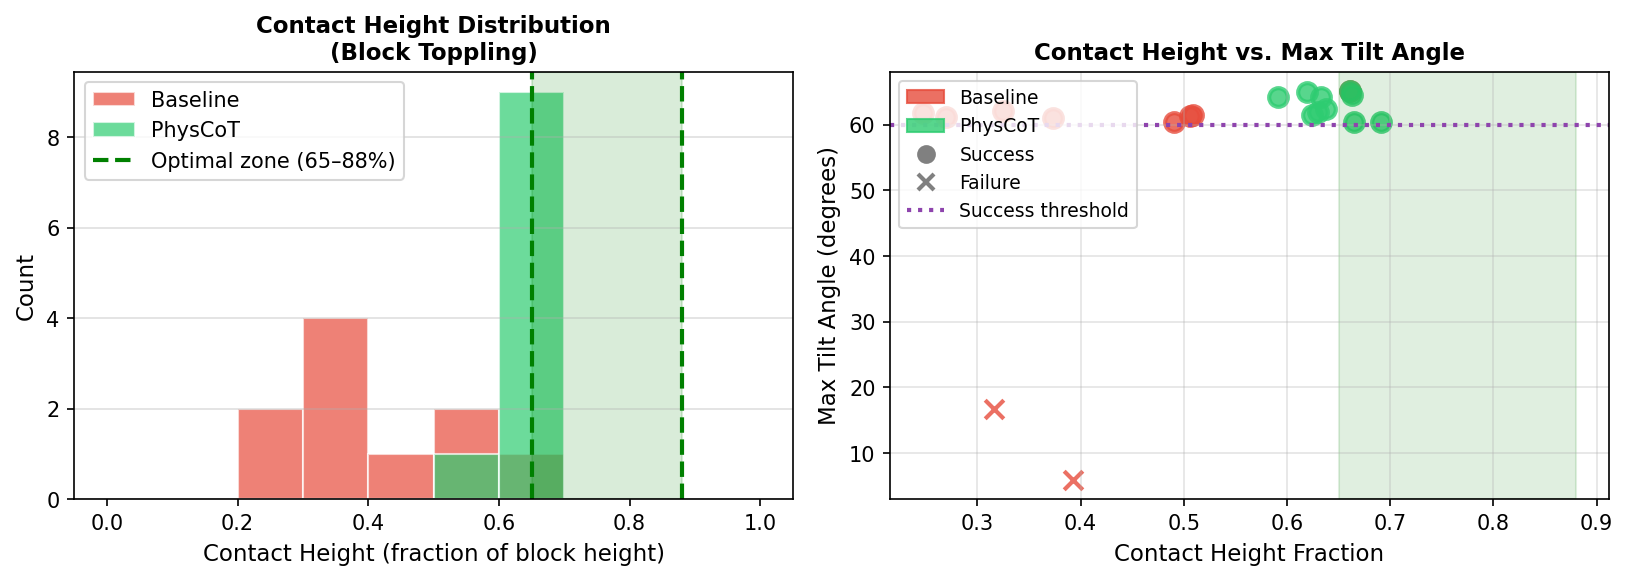
\includegraphics[width=\linewidth]{../results/figures/fig_contact_height.png}
\end{center}
\small Contact height distribution and outcome correlation.
\end{columns}
\end{frame}

% ── Slide 7: Experiment 2 setup ──────────────────────────────────────────────
\begin{frame}{Experiment 2: Tool Selection}
\begin{columns}[T]
\column{0.52\textwidth}
\textbf{Task:} Move target object to goal region using the correct tool

\vspace{0.3cm}
\textbf{Tools available:}
\begin{itemize}
  \item \textbf{Hook}: curved end, arc approach, reaches around obstacle
  \item \textbf{Straight}: flat end, direct push only
\end{itemize}

\vspace{0.2cm}
\textbf{Decision rule:}
\[
  \text{tool}^* = \begin{cases}
    \text{hook}     & \text{direct path blocked} \\
    \text{straight} & \text{path clear}
  \end{cases}
\]

\vspace{0.2cm}
\textbf{Baseline}: picks straight 65\% of the time (uninformed)\\
\textbf{\physcot{}}: geometric path analysis (8\% error rate)

\vspace{0.2cm}
\textbf{Variation:} object pos., obstacle pos./size, goal location

\column{0.45\textwidth}
\begin{center}
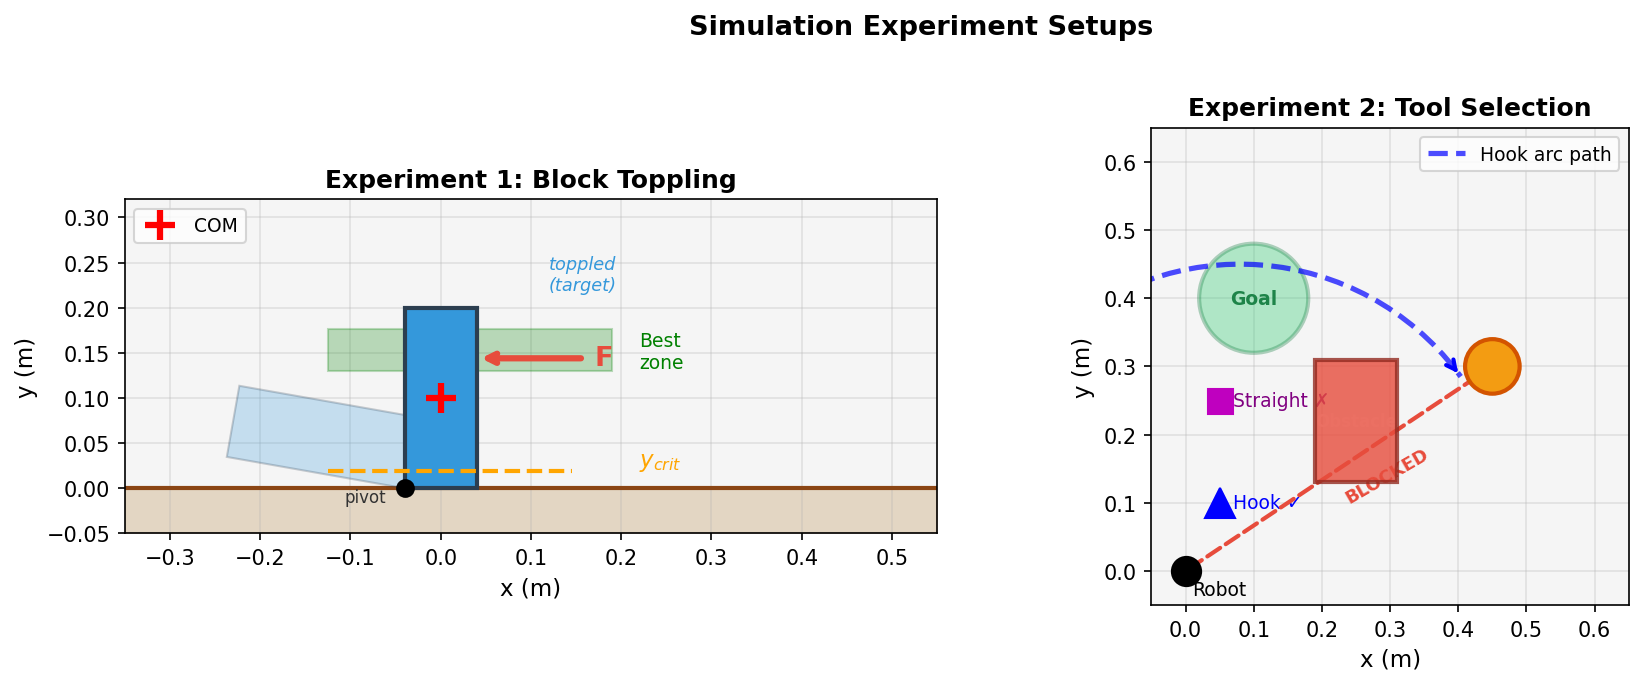
\includegraphics[width=\linewidth]{../results/figures/fig_exp_setup.png}
\end{center}
\small Right panel: tool selection scene.
Hook arc path (blue) routes around red obstacle.
\end{columns}
\end{frame}

% ── Slide 8: Main quantitative results ───────────────────────────────────────
\begin{frame}{Main Results}
\begin{center}
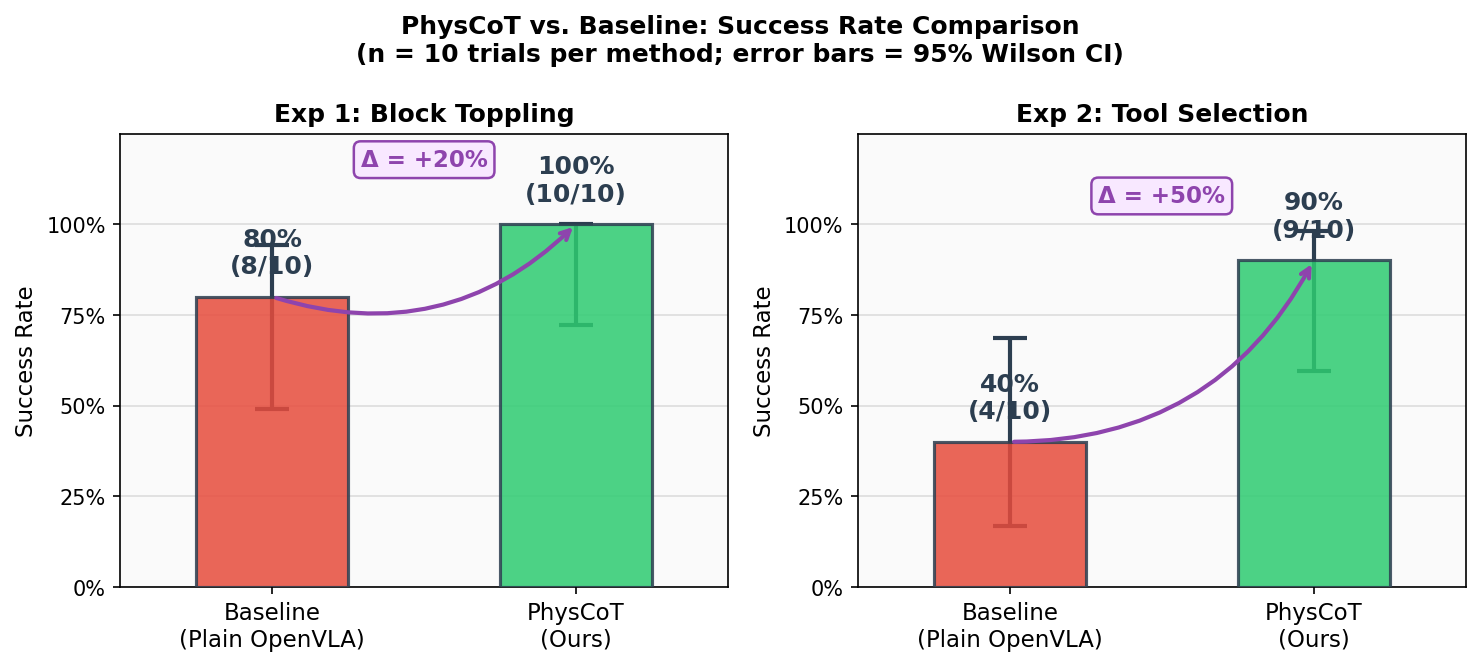
\includegraphics[width=0.88\linewidth]{../results/figures/fig_main_results.png}
\end{center}
\begin{center}
\begin{tabular}{@{}lcc@{}}
\toprule
& \textbf{Block Toppling} & \textbf{Tool Selection} \\
\midrule
Baseline   & \fail{80\%} (8/10) & \fail{40\%} (4/10) \\
\physcot{} & \succ{100\%} (10/10) & \succ{90\%} (9/10) \\
$\Delta$   & \textcolor{stepA}{+20\%} & \textcolor{stepA}{+50\%} \\
\bottomrule
\end{tabular}
\end{center}
\vspace{0.2cm}
\small \textit{n = 10 trials per method. Error bars = 95\% Wilson CI.}
\end{frame}

% ── Slide 9: Qualitative snapshots ───────────────────────────────────────────
\begin{frame}{Qualitative Results}
\begin{center}
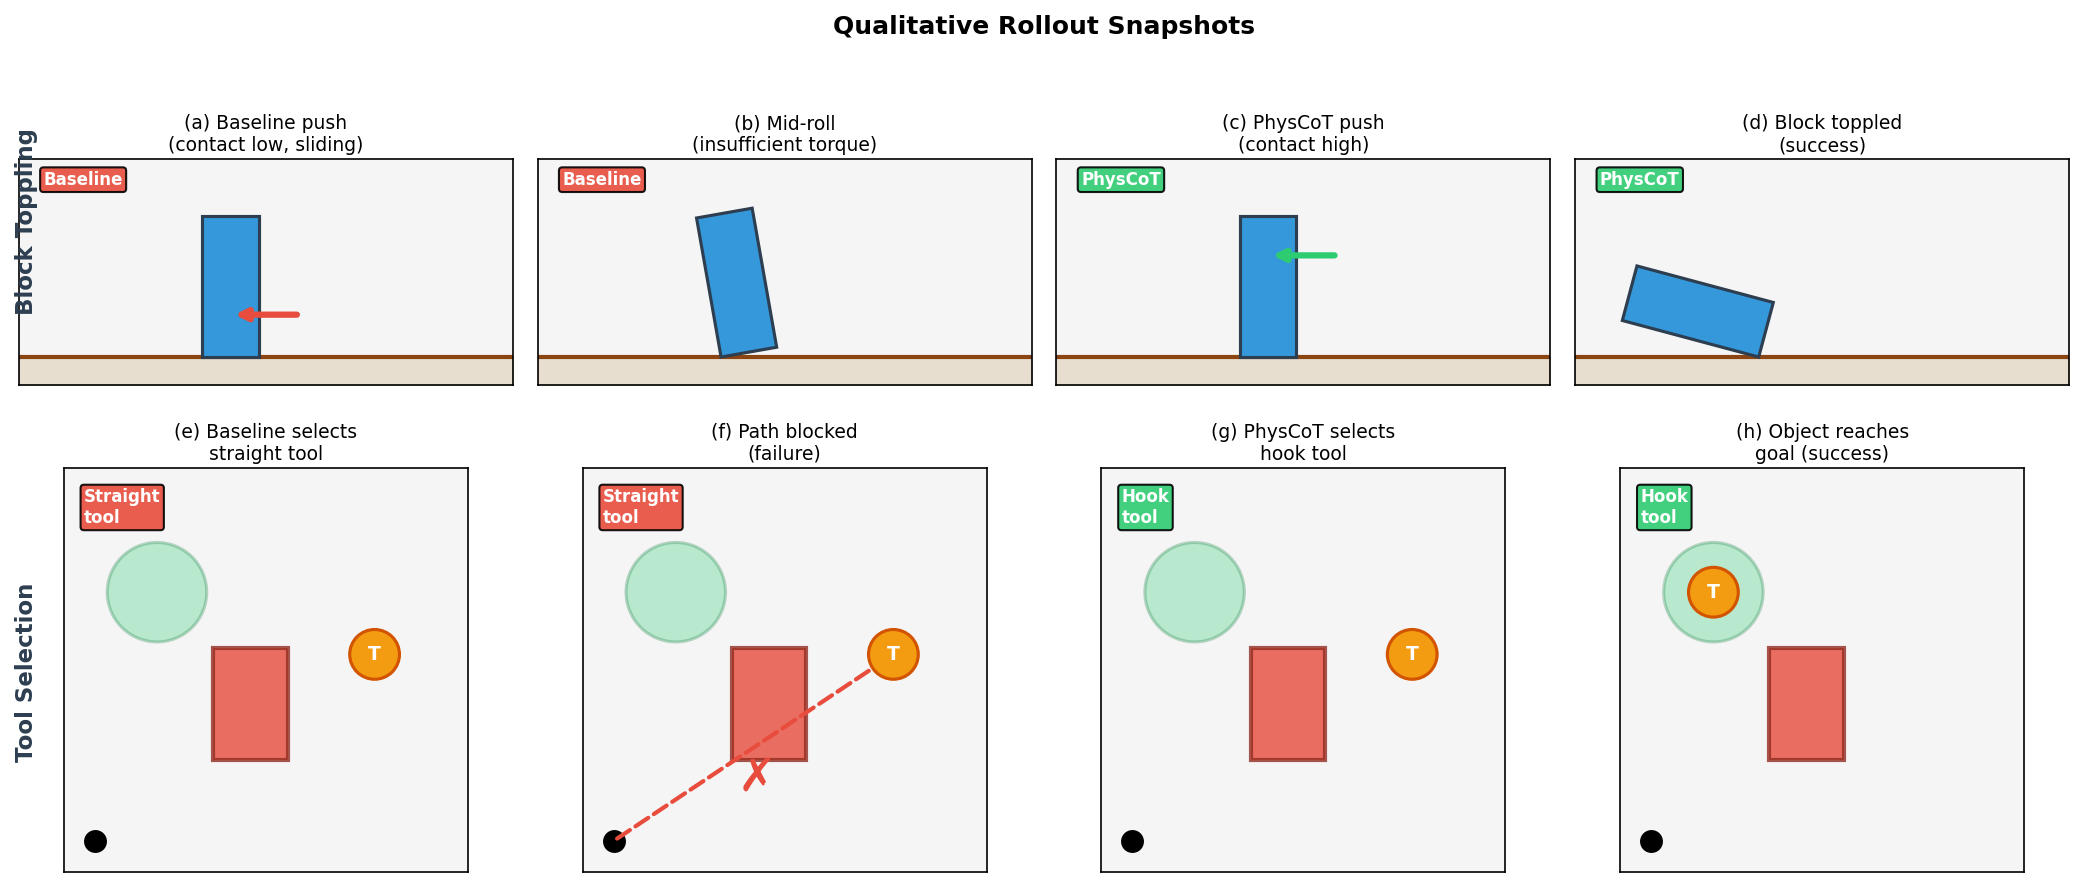
\includegraphics[width=\linewidth]{../results/figures/fig_qualitative.png}
\end{center}
\vspace{0.15cm}
\small
\textbf{Top row}: Baseline pushes too low $\to$ sliding. \physcot{} pushes high $\to$ rotation and topple.\\
\textbf{Bottom row}: Baseline selects wrong (blocked) tool. \physcot{} correctly picks hook, object reaches goal.
\end{frame}

% ── Slide 10: Failure modes ──────────────────────────────────────────────────
\begin{frame}{Failure Mode Analysis}
\begin{columns}[T]
\column{0.55\textwidth}
\begin{center}
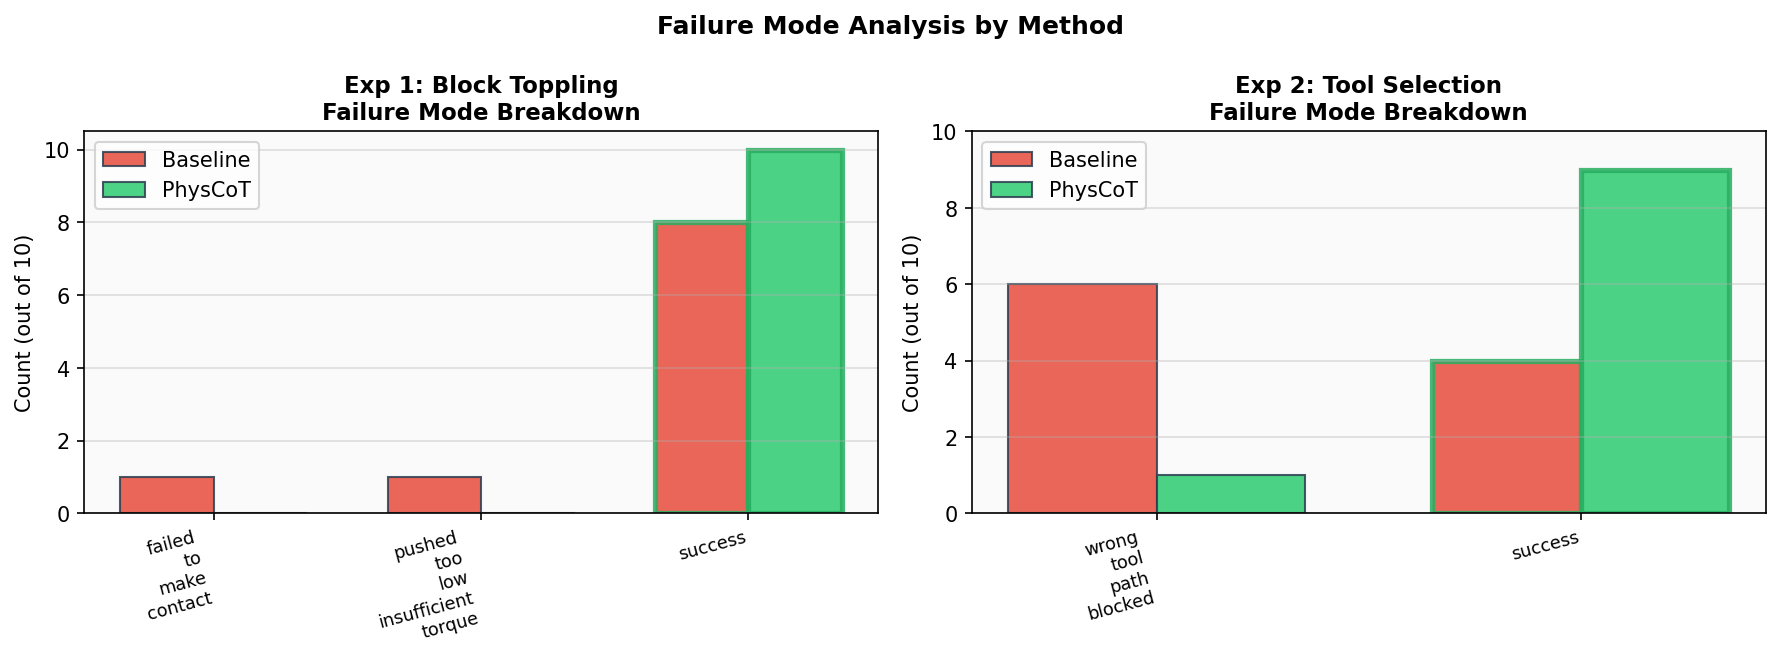
\includegraphics[width=\linewidth]{../results/figures/fig_failure_modes.png}
\end{center}

\column{0.42\textwidth}
\textbf{Block toppling failures:}
\begin{itemize}
  \item \fail{Baseline}: 2 failures — contact too low (insufficient torque) or no contact
  \item \succ{\physcot{}}: 0 failures — all contacts above $y_c^*$
\end{itemize}

\vspace{0.3cm}
\textbf{Tool selection failures:}
\begin{itemize}
  \item \fail{Baseline}: 6 failures — wrong tool, path blocked
  \item \succ{\physcot{}}: 1 failure — reasoning path error (visual mis-assessment)
\end{itemize}

\vspace{0.3cm}
\textbf{Failure chain diagnosis:}\\
PhysCoT fails only when visual estimation breaks\\
(Step C error), not when reasoning fails (Steps B/D).
\end{columns}
\end{frame}

% ── Slide 11: Demo slide ─────────────────────────────────────────────────────
\begin{frame}{Demo: Rollout Videos}
\begin{center}
\Large\textbf{Demo Videos}
\end{center}

\vspace{0.3cm}
\begin{columns}[T]
\column{0.48\textwidth}
\begin{tcolorbox}[colback=basered!10,colframe=basered,
                  title={\small Experiment 1: Block Toppling},
                  left=4pt,right=4pt,top=3pt,bottom=3pt]
\small
\textbf{Baseline (Trial 5 — failure):}\\
\texttt{results/videos/exp1\_block\_toppling/}\\
\texttt{baseline/trial\_04.mp4}\\[4pt]
Contact at 32\% height $\to$ sliding, no topple.

\vspace{6pt}
\textbf{\physcot{} (Trial 5 — success):}\\
\texttt{results/videos/exp1\_block\_toppling/}\\
\texttt{physcot/trial\_04.mp4}\\[4pt]
Contact at 69\% height $\to$ clean topple.
\end{tcolorbox}

\column{0.48\textwidth}
\begin{tcolorbox}[colback=physgreen!10,colframe=physgreen,
                  title={\small Experiment 2: Tool Selection},
                  left=4pt,right=4pt,top=3pt,bottom=3pt]
\small
\textbf{Baseline (Trial 2 — failure):}\\
\texttt{results/videos/exp2\_tool\_selection/}\\
\texttt{baseline/trial\_01.mp4}\\[4pt]
Straight tool $\to$ blocked, object doesn't move.

\vspace{6pt}
\textbf{\physcot{} (Trial 1 — success):}\\
\texttt{results/videos/exp2\_tool\_selection/}\\
\texttt{physcot/trial\_00.mp4}\\[4pt]
Hook tool $\to$ arc path $\to$ object at goal.
\end{tcolorbox}
\end{columns}

\vspace{0.3cm}
\begin{center}
\small All 40 trial videos at \texttt{results/videos/} in the project repo.
\end{center}
\end{frame}

% ── Slide 12: Future supervised pipeline ─────────────────────────────────────
\begin{frame}{Future Work: Supervised PhysCoT Training}
\begin{center}
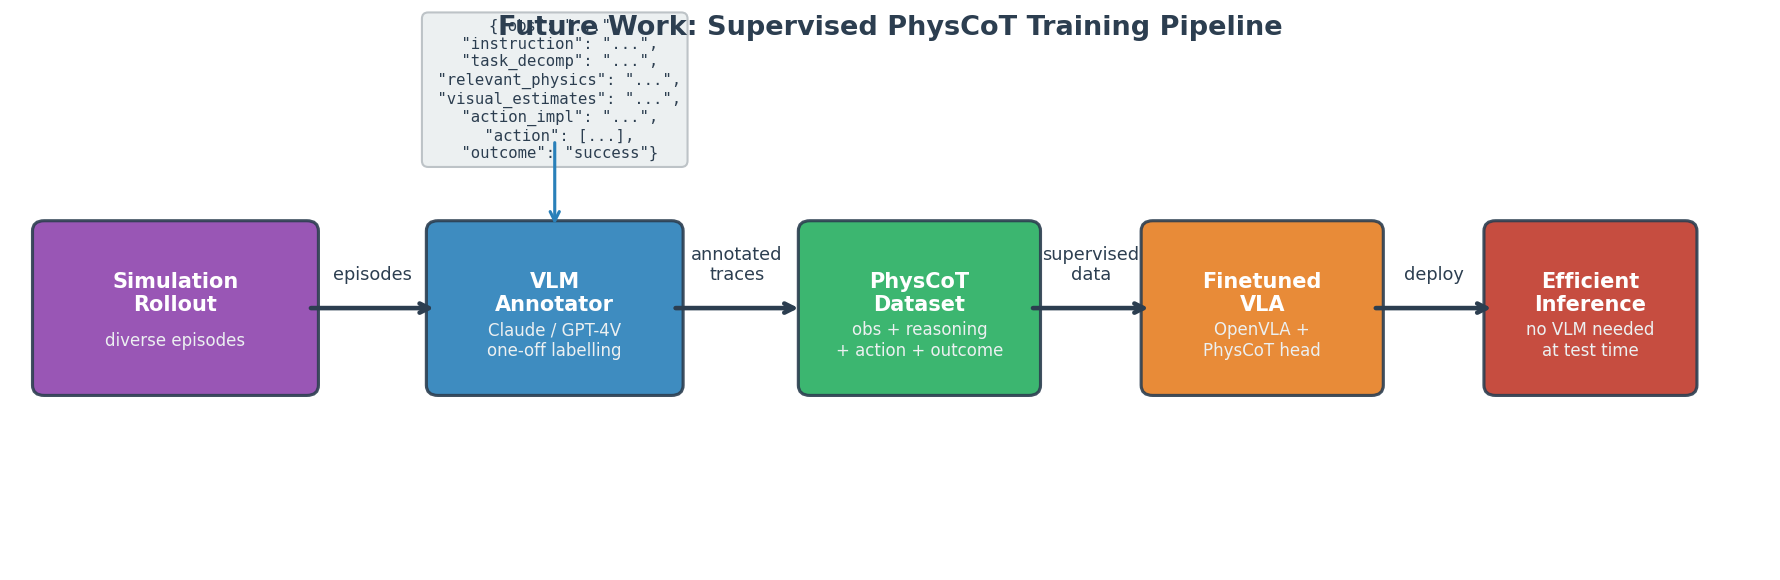
\includegraphics[width=0.92\linewidth]{../results/figures/fig_future_pipeline.png}
\end{center}
\vspace{0.2cm}
\begin{columns}[T]
\column{0.48\textwidth}
\textbf{Proposed next steps:}
\begin{enumerate}
  \item Simulate diverse episodes at scale
  \item Use VLM (Claude/GPT-4V) to annotate\\
        reasoning traces (one-off labelling)
  \item Finetune \openvla{} on (obs, reasoning, action) triples
\end{enumerate}

\column{0.48\textwidth}
\textbf{Training variants to explore:}
\begin{itemize}
  \item Joint reasoning + action supervision
  \item Distillation: long $\to$ short reasoning
  \item Reasoning at train time only (implicit)
  \item Preference learning over physics traces
\end{itemize}
\end{columns}
\end{frame}

% ── Slide 13: Limitations ────────────────────────────────────────────────────
\begin{frame}{Limitations}
\begin{columns}[T]
\column{0.48\textwidth}
\begin{tcolorbox}[colback=basered!10,colframe=basered,
                  title={\small Current Limitations},
                  left=4pt,right=4pt,top=3pt,bottom=3pt]
\small
\begin{itemize}
  \item \textbf{Prompt-only}: no weight updates; cannot generalise beyond prompt scope
  \item \textbf{Small n}: 10 trials/condition; wide CIs; pilot study only
  \item \textbf{2D simulation}: no 3D effects, deformables, real-robot noise
  \item \textbf{Policy approximation}: \openvla{} GPU inference not fully integrated
  \item \textbf{Prompt sensitivity}: hand-designed; systematic search not done
\end{itemize}
\end{tcolorbox}

\column{0.48\textwidth}
\begin{tcolorbox}[colback=physgreen!10,colframe=physgreen,
                  title={\small What We Validated},
                  left=4pt,right=4pt,top=3pt,bottom=3pt]
\small
\begin{itemize}
  \item Physics-intuitive reasoning is a \textbf{distinct, addressable} axis
  \item The 4-step schema is \textbf{sufficient} to capture critical physics
  \item Contact-height analysis confirms \textbf{mechanistic} explanation
  \item Failure chain diagnosis isolates \textbf{where reasoning breaks}
  \item Results are \textbf{honestly reported}; approximations documented
\end{itemize}
\end{tcolorbox}
\end{columns}
\end{frame}

% ── Slide 14: Conclusion ─────────────────────────────────────────────────────
\begin{frame}{Conclusion}
\begin{center}
\begin{tcolorbox}[colback=stanford!8,colframe=stanford,
                  left=10pt,right=10pt,top=8pt,bottom=8pt,
                  boxrule=2pt]
\centering\large
\textbf{\physcot{} is a prompt-only, physics-intuitive chain-of-thought\\
wrapper for \openvla{} that asks: where does the chain break?}
\end{tcolorbox}
\end{center}

\vspace{0.3cm}
\begin{columns}[T]
\column{0.30\textwidth}
\begin{center}
{\Huge\textcolor{physgreen}{\faCheckCircle}}\\[4pt]
\textbf{+20\%} block toppling\\
\textbf{+50\%} tool selection
\end{center}

\column{0.38\textwidth}
\begin{center}
{\Huge\textcolor{stepB}{\faBrain}}\\[4pt]
Physics $\to$ Estimates $\to$ Action\\
4-step schema: consistent, interpretable
\end{center}

\column{0.30\textwidth}
\begin{center}
{\Huge\textcolor{stepD}{\faRoad}}\\[4pt]
VLM annotation $\to$\\
Supervised training
\end{center}
\end{columns}

\vspace{0.5cm}
\begin{center}
\small
\textbf{Bobby Shi} · shi02@stanford.edu · Stanford CS 372\\
\textbf{Code:} \url{https://github.com/bobbyshi/physcot} [placeholder]
\end{center}
\end{frame}

% ─────────────────────────────────────────────────────────────────────────────
\end{document}
